  \documentclass{beamer}
    \usepackage[utf8]{inputenc}
    
    \usetheme{Madrid}
    \usecolortheme{default}
    \usepackage{amsmath,amssymb,amsfonts,amsthm}
    \usepackage{mathtools}
    \usepackage{txfonts}
    \usepackage{tkz-euclide}
    \usepackage{listings}
    \usepackage{adjustbox}
    \usepackage{array}
    \usepackage{gensymb}
    \usepackage{tabularx}
    \usepackage{gvv}
    \usepackage{lmodern}
    \usepackage{circuitikz}
    \usepackage{tikz}
    \lstset{literate={·}{{$\cdot$}}1 {λ}{{$\lambda$}}1 {→}{{$\to$}}1}
    \usepackage{graphicx}
    
    \setbeamertemplate{page number in head/foot}[totalframenumber]
    
    \usepackage{tcolorbox}
    \tcbuselibrary{minted,breakable,xparse,skins}
    
    
    
    \definecolor{bg}{gray}{0.95}
    \DeclareTCBListing{mintedbox}{O{}m!O{}}{%
      breakable=true,
      listing engine=minted,
      listing only,
      minted language=#2,
      minted style=default,
      minted options={%
        linenos,
        gobble=0,
        breaklines=true,
        breakafter=,,
        fontsize=\small,
        numbersep=8pt,
        #1},
      boxsep=0pt,
      left skip=0pt,
      right skip=0pt,
      left=25pt,
      right=0pt,
      top=3pt,
      bottom=3pt,
      arc=5pt,
      leftrule=0pt,
      rightrule=0pt,
      bottomrule=2pt,
      toprule=2pt,
      colback=bg,
      colframe=orange!70,
      enhanced,
      overlay={%
        \begin{tcbclipinterior}
        \fill[orange!20!white] (frame.south west) rectangle ([xshift=20pt]frame.north west);
        \end{tcbclipinterior}},
      #3,
    }
    \lstset{
        language=C,
        basicstyle=\ttfamily\small,
        keywordstyle=\color{blue},
        stringstyle=\color{orange},
        commentstyle=\color{green!60!black},
        numbers=left,
        numberstyle=\tiny\color{gray},
        breaklines=true,
        showstringspaces=false,
    }
    %------------------------------------------------------------
    %This block of code defines the information to appear in the
    %Title page
    \title %optional
    {7.4.34}
    \date{30 September, 2025}
    %\subtitle{A short story}
    
    \author % (optional)
    {INDHIRESH S - EE25BTECH11027}
    
    \begin{document}
    
    \frame{\titlepage}
    
    \begin{frame}{Question}
      Find the equation of the circle whose radius is 5 and which touches the circle $x^2 +y^2 - 2x - 4y - 20 = 0$ at the point $(5, 5)$.
    \end{frame}
    
    \begin{frame}[allowframebreaks] 
    \frametitle{Equation}
        \centering
        \label{tab:parameters}
   The general circle equation can be given as:
\begin{align}
  \norm{\Vec{x}}^2+2\Vec{u^T}\Vec{x}+f=0
\end{align}
Let the equation of the first circle be

\begin{align}
  \norm{\Vec{x}}^2+2\Vec{u_1^T}\Vec{x}+f_1=0
\end{align}
The equation of the second circle be:
\begin{align}
    \norm{\Vec{x}}^2+2\Vec{u_2^T}\Vec{x}+f_2=0
\end{align}
    \end{frame}
    
    \begin{frame}
    \frametitle{Theoretical Solution}
From the given information:
\begin{align}
   \Vec{u_1}=\myvec{-1\\-2}\;\;and\;\;f_1=-20
\end{align}
Let $\Vec{c_1}$ and $\Vec{c_2}$ be the centre of the circle 1 and circle 2:
\begin{align}
  \Vec{c_1}=\Vec{-u_1}=\myvec{1\\2}
\end{align}
And also
\begin{align}
   f_1=\norm{\Vec{u_1}}^2-r_1
\end{align}

\begin{align}
  r_1=5
\end{align}

    \end{frame}
    
    \begin{frame}
    \frametitle{Theoretical solution}
   Let P be the point of contact
\begin{align}
    \Vec{P}=\myvec{5\\5}
\end{align}
If the two circle touch each other externally at $\Vec{P}$. So the $\Vec{P},\Vec{c_1}$ and $\Vec{c_2}$ will be collinear and $\Vec{P}$ will divide the points $\Vec{c_1}$ and $\Vec{c_2}$ in the ratio $\frac{r_1}{r_2}:1$
\begin{align}
   \frac{r_1}{r_2}=1
\end{align}
\begin{align}
   \Vec{P}=\frac{\Vec{c_1}+\Vec{c_2}}{2}
\end{align}
\begin{align}
    \myvec{5\\5}=\frac{\myvec{1\\2}+\Vec{c_2}}{2}
\end{align}

    \end{frame}
    
    \begin{frame}
    \frametitle{Theoretical Solution}
    \begin{align}
\Vec{c_2}=\myvec{9\\8}
  \end{align}
If two circles touch each other internally we get:

\begin{align}
 \Vec{c_2}=\myvec{1\\2}
\end{align}
This is the same as circle 1, so the two circles touch each other externally.\\
Now
\begin{align}
    r_2=5\;\;and\;\;\Vec{c_2}=\myvec{9\\8}
\end{align}
\begin{align}
\Vec{u_2}=\Vec{-c_2}=\myvec{-9\\-8}
\end{align}


    \end{frame}
    
    \begin{frame}
    \frametitle{Theoretical Solution}
   \begin{align}
    f_2=\norm{\Vec{u_2}}^2-r_2
\end{align}
\begin{align}
   f_2=120
\end{align}
Now the required equation of circle is
\begin{align}
   \norm{\Vec{x}}^2+2\Vec{u_2^T}\Vec{x}+f_2=0
\end{align}
\begin{align}
    \norm{\Vec{x}}^2+2\myvec{-9\\-8}^Tx+120=0
\end{align}
    \end{frame}
    
   
    
    \begin{frame}[fragile]
        \frametitle{C Code}
        \begin{lstlisting}
    #include <math.h>

typedef struct {
    double x;
    double y;
} Point;

void solve_circle_tangency(double G1, double H1, double K1, Point p, double r2, Point* c1_center_out, Point* c2_center_out) {
    double c1_x = -G1 / 2.0;
    double c1_y = -H1 / 2.0;
    double m_x = p.x - c1_x;
    double m_y = p.y - c1_y;
    double mag_m = sqrt(m_x * m_x + m_y * m_y);
    double m_hat_x = m_x / mag_m;
    double m_hat_y = m_y / mag_m;
   
        \end{lstlisting}
    \end{frame}
    
    \begin{frame}[fragile]
        \frametitle{C Code}
        \begin{lstlisting}
       c1_center_out->x = c1_x;
    c1_center_out->y = c1_y;
    c2_center_out->x = p.x + r2 * m_hat_x;
    c2_center_out->y = p.y + r2 * m_hat_y;
}
        \end{lstlisting}
    \end{frame}
    
    
    \begin{frame}[fragile]
        \frametitle{Python Code}
        \begin{lstlisting}
import ctypes
import numpy as np
import matplotlib.pyplot as plt

# Define a ctypes Structure that mirrors the C struct
class Point(ctypes.Structure):
    _fields_ = [("x", ctypes.c_double),
                ("y", ctypes.c_double)]

# --- Load the C library ---
c_lib = ctypes.CDLL('./circle.so')

# --- Define the C function's argument and return types ---
c_lib.solve_circle_tangency.argtypes = [
    ctypes.c_double, ctypes.c_double, ctypes.c_double,
    Point, ctypes.c_double,
    ctypes.POINTER(Point), ctypes.POINTER(Point)
]

        \end{lstlisting}
    \end{frame}
    
    \begin{frame}[fragile]
        \frametitle{Python Code}
        \begin{lstlisting}
   c_lib.solve_circle_tangency.restype = None

# --- Numerical Inputs are defined in Python using NumPy ---
G1, H1, K1 = -2.0, -4.0, -20.0
p_tangency_np = np.array([5.0, 5.0])
r1, r2 = 5.0, 5.0
# ---------------------------------------------------------

# --- Prepare data for C function call ---
# 1. Convert NumPy array to the ctypes Point structure
p_tangency_ctypes = Point(x=p_tangency_np[0], y=p_tangency_np[1])

# 2. Prepare empty ctypes structures to receive the output
c1_center_ctypes = Point()
c2_center_ctypes = Point()


        \end{lstlisting}
    \end{frame}
    
    \begin{frame}[fragile]
        \frametitle{Python Code}
        \begin{lstlisting}
   # --- Call the C function ---
c_lib.solve_circle_tangency(
    G1, H1, K1, p_tangency_ctypes, r2, 
    ctypes.byref(c1_center_ctypes), 
    ctypes.byref(c2_center_ctypes)
)

# --- Convert results from ctypes back to NumPy arrays ---
c1 = np.array([c1_center_ctypes.x, c1_center_ctypes.y])
c2 = np.array([c2_center_ctypes.x, c2_center_ctypes.y])
p = p_tangency_np # Use the original numpy array

# --- Plotting with NumPy arrays ---
fig, ax = plt.subplots(figsize=(8, 8))


        \end{lstlisting}
    \end{frame}
    
    \begin{frame}[fragile]
        \frametitle{Python Code}
        \begin{lstlisting}
    # Plot the circles
circle1 = plt.Circle(c1, r1, fill=False, edgecolor='gray', linestyle='--')
circle2 = plt.Circle(c2, r2, fill=False, edgecolor='gray', linestyle='-')
ax.add_patch(circle1)
ax.add_patch(circle2)

# Plot the line connecting centers
ax.plot([c1[0], c2[0]], [c1[1], c2[1]], 'b-', label='Line of Centers')

# Plot the key points
ax.plot(c1[0], c1[1], 'ro', markersize=10, label=f'C1({c1[0]:.2f}, {c1[1]:.2f})')
ax.plot(c2[0], c2[1], 'go', markersize=10, label=f'C2({c2[0]:.2f}, {c2[1]:.2f})')

        \end{lstlisting}
    \end{frame}

     \begin{frame}[fragile]
        \frametitle{Python Code}
        \begin{lstlisting}
    ax.plot(p[0], p[1], 'm*', markersize=15, label=f'P({p[0]:.2f}, {p[1]:.2f})')

ax.text(c1[0] + 0.2, c1[1] + 0.2, 'C1', fontsize=12, color='red', fontweight='bold')
ax.text(c2[0] + 0.2, c2[1] + 0.2, 'C2', fontsize=12, color='green', fontweight='bold')
ax.text(p[0] + 0.2, p[1] + 0.2, 'P', fontsize=12, color='magenta', fontweight='bold')

# Formatting
ax.set_title('Figure')
ax.grid(True)
ax.axis('equal')
ax.legend()
plt.savefig("/media/indhiresh-s/New Volume/Matrix/ee1030-2025/ee25btech11027/MATGEO/7.4.34/figs/figure1.png")
plt.show()
        \end{lstlisting}
    \end{frame}
    
    \begin{frame}{Plot}
        \begin{center}
            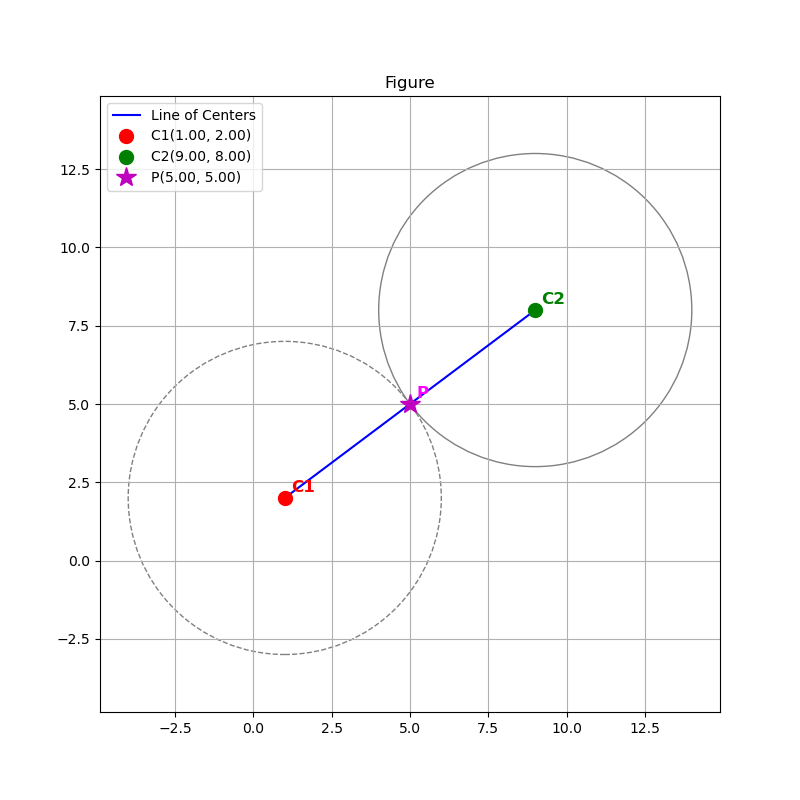
\includegraphics[width=\columnwidth, height=0.8\textheight, keepaspectratio]{figs/figure1.png}
        \end{center}
    \end{frame}
    
    \end{document}